% Options for packages loaded elsewhere
\PassOptionsToPackage{unicode}{hyperref}
\PassOptionsToPackage{hyphens}{url}
\PassOptionsToPackage{dvipsnames,svgnames,x11names}{xcolor}
%
\documentclass[
  letterpaper,
  DIV=11,
  numbers=noendperiod]{scrreprt}

\usepackage{amsmath,amssymb}
\usepackage{lmodern}
\usepackage{iftex}
\ifPDFTeX
  \usepackage[T1]{fontenc}
  \usepackage[utf8]{inputenc}
  \usepackage{textcomp} % provide euro and other symbols
\else % if luatex or xetex
  \usepackage{unicode-math}
  \defaultfontfeatures{Scale=MatchLowercase}
  \defaultfontfeatures[\rmfamily]{Ligatures=TeX,Scale=1}
\fi
% Use upquote if available, for straight quotes in verbatim environments
\IfFileExists{upquote.sty}{\usepackage{upquote}}{}
\IfFileExists{microtype.sty}{% use microtype if available
  \usepackage[]{microtype}
  \UseMicrotypeSet[protrusion]{basicmath} % disable protrusion for tt fonts
}{}
\makeatletter
\@ifundefined{KOMAClassName}{% if non-KOMA class
  \IfFileExists{parskip.sty}{%
    \usepackage{parskip}
  }{% else
    \setlength{\parindent}{0pt}
    \setlength{\parskip}{6pt plus 2pt minus 1pt}}
}{% if KOMA class
  \KOMAoptions{parskip=half}}
\makeatother
\usepackage{xcolor}
\setlength{\emergencystretch}{3em} % prevent overfull lines
\setcounter{secnumdepth}{5}
% Make \paragraph and \subparagraph free-standing
\ifx\paragraph\undefined\else
  \let\oldparagraph\paragraph
  \renewcommand{\paragraph}[1]{\oldparagraph{#1}\mbox{}}
\fi
\ifx\subparagraph\undefined\else
  \let\oldsubparagraph\subparagraph
  \renewcommand{\subparagraph}[1]{\oldsubparagraph{#1}\mbox{}}
\fi

\usepackage{color}
\usepackage{fancyvrb}
\newcommand{\VerbBar}{|}
\newcommand{\VERB}{\Verb[commandchars=\\\{\}]}
\DefineVerbatimEnvironment{Highlighting}{Verbatim}{commandchars=\\\{\}}
% Add ',fontsize=\small' for more characters per line
\usepackage{framed}
\definecolor{shadecolor}{RGB}{241,243,245}
\newenvironment{Shaded}{\begin{snugshade}}{\end{snugshade}}
\newcommand{\AlertTok}[1]{\textcolor[rgb]{0.68,0.00,0.00}{#1}}
\newcommand{\AnnotationTok}[1]{\textcolor[rgb]{0.37,0.37,0.37}{#1}}
\newcommand{\AttributeTok}[1]{\textcolor[rgb]{0.40,0.45,0.13}{#1}}
\newcommand{\BaseNTok}[1]{\textcolor[rgb]{0.68,0.00,0.00}{#1}}
\newcommand{\BuiltInTok}[1]{\textcolor[rgb]{0.00,0.23,0.31}{#1}}
\newcommand{\CharTok}[1]{\textcolor[rgb]{0.13,0.47,0.30}{#1}}
\newcommand{\CommentTok}[1]{\textcolor[rgb]{0.37,0.37,0.37}{#1}}
\newcommand{\CommentVarTok}[1]{\textcolor[rgb]{0.37,0.37,0.37}{\textit{#1}}}
\newcommand{\ConstantTok}[1]{\textcolor[rgb]{0.56,0.35,0.01}{#1}}
\newcommand{\ControlFlowTok}[1]{\textcolor[rgb]{0.00,0.23,0.31}{#1}}
\newcommand{\DataTypeTok}[1]{\textcolor[rgb]{0.68,0.00,0.00}{#1}}
\newcommand{\DecValTok}[1]{\textcolor[rgb]{0.68,0.00,0.00}{#1}}
\newcommand{\DocumentationTok}[1]{\textcolor[rgb]{0.37,0.37,0.37}{\textit{#1}}}
\newcommand{\ErrorTok}[1]{\textcolor[rgb]{0.68,0.00,0.00}{#1}}
\newcommand{\ExtensionTok}[1]{\textcolor[rgb]{0.00,0.23,0.31}{#1}}
\newcommand{\FloatTok}[1]{\textcolor[rgb]{0.68,0.00,0.00}{#1}}
\newcommand{\FunctionTok}[1]{\textcolor[rgb]{0.28,0.35,0.67}{#1}}
\newcommand{\ImportTok}[1]{\textcolor[rgb]{0.00,0.46,0.62}{#1}}
\newcommand{\InformationTok}[1]{\textcolor[rgb]{0.37,0.37,0.37}{#1}}
\newcommand{\KeywordTok}[1]{\textcolor[rgb]{0.00,0.23,0.31}{#1}}
\newcommand{\NormalTok}[1]{\textcolor[rgb]{0.00,0.23,0.31}{#1}}
\newcommand{\OperatorTok}[1]{\textcolor[rgb]{0.37,0.37,0.37}{#1}}
\newcommand{\OtherTok}[1]{\textcolor[rgb]{0.00,0.23,0.31}{#1}}
\newcommand{\PreprocessorTok}[1]{\textcolor[rgb]{0.68,0.00,0.00}{#1}}
\newcommand{\RegionMarkerTok}[1]{\textcolor[rgb]{0.00,0.23,0.31}{#1}}
\newcommand{\SpecialCharTok}[1]{\textcolor[rgb]{0.37,0.37,0.37}{#1}}
\newcommand{\SpecialStringTok}[1]{\textcolor[rgb]{0.13,0.47,0.30}{#1}}
\newcommand{\StringTok}[1]{\textcolor[rgb]{0.13,0.47,0.30}{#1}}
\newcommand{\VariableTok}[1]{\textcolor[rgb]{0.07,0.07,0.07}{#1}}
\newcommand{\VerbatimStringTok}[1]{\textcolor[rgb]{0.13,0.47,0.30}{#1}}
\newcommand{\WarningTok}[1]{\textcolor[rgb]{0.37,0.37,0.37}{\textit{#1}}}

\providecommand{\tightlist}{%
  \setlength{\itemsep}{0pt}\setlength{\parskip}{0pt}}\usepackage{longtable,booktabs,array}
\usepackage{calc} % for calculating minipage widths
% Correct order of tables after \paragraph or \subparagraph
\usepackage{etoolbox}
\makeatletter
\patchcmd\longtable{\par}{\if@noskipsec\mbox{}\fi\par}{}{}
\makeatother
% Allow footnotes in longtable head/foot
\IfFileExists{footnotehyper.sty}{\usepackage{footnotehyper}}{\usepackage{footnote}}
\makesavenoteenv{longtable}
\usepackage{graphicx}
\makeatletter
\def\maxwidth{\ifdim\Gin@nat@width>\linewidth\linewidth\else\Gin@nat@width\fi}
\def\maxheight{\ifdim\Gin@nat@height>\textheight\textheight\else\Gin@nat@height\fi}
\makeatother
% Scale images if necessary, so that they will not overflow the page
% margins by default, and it is still possible to overwrite the defaults
% using explicit options in \includegraphics[width, height, ...]{}
\setkeys{Gin}{width=\maxwidth,height=\maxheight,keepaspectratio}
% Set default figure placement to htbp
\makeatletter
\def\fps@figure{htbp}
\makeatother
\newlength{\cslhangindent}
\setlength{\cslhangindent}{1.5em}
\newlength{\csllabelwidth}
\setlength{\csllabelwidth}{3em}
\newlength{\cslentryspacingunit} % times entry-spacing
\setlength{\cslentryspacingunit}{\parskip}
\newenvironment{CSLReferences}[2] % #1 hanging-ident, #2 entry spacing
 {% don't indent paragraphs
  \setlength{\parindent}{0pt}
  % turn on hanging indent if param 1 is 1
  \ifodd #1
  \let\oldpar\par
  \def\par{\hangindent=\cslhangindent\oldpar}
  \fi
  % set entry spacing
  \setlength{\parskip}{#2\cslentryspacingunit}
 }%
 {}
\usepackage{calc}
\newcommand{\CSLBlock}[1]{#1\hfill\break}
\newcommand{\CSLLeftMargin}[1]{\parbox[t]{\csllabelwidth}{#1}}
\newcommand{\CSLRightInline}[1]{\parbox[t]{\linewidth - \csllabelwidth}{#1}\break}
\newcommand{\CSLIndent}[1]{\hspace{\cslhangindent}#1}

\KOMAoption{captions}{tableheading}
\makeatletter
\makeatother
\makeatletter
\@ifpackageloaded{bookmark}{}{\usepackage{bookmark}}
\makeatother
\makeatletter
\@ifpackageloaded{caption}{}{\usepackage{caption}}
\AtBeginDocument{%
\ifdefined\contentsname
  \renewcommand*\contentsname{Table of contents}
\else
  \newcommand\contentsname{Table of contents}
\fi
\ifdefined\listfigurename
  \renewcommand*\listfigurename{List of Figures}
\else
  \newcommand\listfigurename{List of Figures}
\fi
\ifdefined\listtablename
  \renewcommand*\listtablename{List of Tables}
\else
  \newcommand\listtablename{List of Tables}
\fi
\ifdefined\figurename
  \renewcommand*\figurename{Figure}
\else
  \newcommand\figurename{Figure}
\fi
\ifdefined\tablename
  \renewcommand*\tablename{Table}
\else
  \newcommand\tablename{Table}
\fi
}
\@ifpackageloaded{float}{}{\usepackage{float}}
\floatstyle{ruled}
\@ifundefined{c@chapter}{\newfloat{codelisting}{h}{lop}}{\newfloat{codelisting}{h}{lop}[chapter]}
\floatname{codelisting}{Listing}
\newcommand*\listoflistings{\listof{codelisting}{List of Listings}}
\makeatother
\makeatletter
\@ifpackageloaded{caption}{}{\usepackage{caption}}
\@ifpackageloaded{subcaption}{}{\usepackage{subcaption}}
\makeatother
\makeatletter
\@ifpackageloaded{tcolorbox}{}{\usepackage[many]{tcolorbox}}
\makeatother
\makeatletter
\@ifundefined{shadecolor}{\definecolor{shadecolor}{rgb}{.97, .97, .97}}
\makeatother
\makeatletter
\makeatother
\ifLuaTeX
  \usepackage{selnolig}  % disable illegal ligatures
\fi
\IfFileExists{bookmark.sty}{\usepackage{bookmark}}{\usepackage{hyperref}}
\IfFileExists{xurl.sty}{\usepackage{xurl}}{} % add URL line breaks if available
\urlstyle{same} % disable monospaced font for URLs
\hypersetup{
  pdftitle={mixed\_models\_guide},
  pdfauthor={Julia Piaskowski},
  colorlinks=true,
  linkcolor={blue},
  filecolor={Maroon},
  citecolor={Blue},
  urlcolor={Blue},
  pdfcreator={LaTeX via pandoc}}

\title{mixed\_models\_guide}
\author{Julia Piaskowski}
\date{8/3/2022}

\begin{document}
\maketitle
\ifdefined\Shaded\renewenvironment{Shaded}{\begin{tcolorbox}[sharp corners, enhanced, borderline west={3pt}{0pt}{shadecolor}, breakable, frame hidden, interior hidden, boxrule=0pt]}{\end{tcolorbox}}\fi

\renewcommand*\contentsname{Table of contents}
{
\hypersetup{linkcolor=}
\setcounter{tocdepth}{2}
\tableofcontents
}
\bookmarksetup{startatroot}

\hypertarget{preface}{%
\chapter*{Preface}\label{preface}}
\addcontentsline{toc}{chapter}{Preface}

This is a defaulf file accompanying a quarto book.

To learn more about Quarto books visit
\url{https://quarto.org/docs/books}.

\bookmarksetup{startatroot}

\hypertarget{introduction}{%
\chapter{Introduction}\label{introduction}}

This guide is focused on frequentist implementations of mixed models in
R. If someone wants to write a Bayesian guide, please go for it! I'm not
experience sufficiently in Bayesian to do this.

Each section contains the minimum to run a model, with more detail found
at the later chapters. Unless I decide it makes more sense to include
early materials.

A Tidymodels framework is used whenever possible because that is a
promising avenue for making the syntax easier to write across packages.

\bookmarksetup{startatroot}

\hypertarget{basic-models}{%
\chapter{Basic Models}\label{basic-models}}

\bookmarksetup{startatroot}

\hypertarget{generalized-linear-mixed-models}{%
\chapter{Generalized Linear Mixed
Models}\label{generalized-linear-mixed-models}}

\begin{Shaded}
\begin{Highlighting}[]
\FunctionTok{library}\NormalTok{(dplyr)}
\end{Highlighting}
\end{Shaded}

\begin{verbatim}

Attaching package: 'dplyr'
\end{verbatim}

\begin{verbatim}
The following objects are masked from 'package:stats':

    filter, lag
\end{verbatim}

\begin{verbatim}
The following objects are masked from 'package:base':

    intersect, setdiff, setequal, union
\end{verbatim}

\begin{Shaded}
\begin{Highlighting}[]
\FunctionTok{library}\NormalTok{(ggplot2)}
\FunctionTok{library}\NormalTok{(glmmTMB)}
\end{Highlighting}
\end{Shaded}

\begin{verbatim}
Warning in checkDepPackageVersion(dep_pkg = "TMB"): Package version inconsistency detected.
glmmTMB was built with TMB version 1.9.0
Current TMB version is 1.9.1
Please re-install glmmTMB from source or restore original 'TMB' package (see '?reinstalling' for more information)
\end{verbatim}

\begin{Shaded}
\begin{Highlighting}[]
\FunctionTok{library}\NormalTok{(DHARMa)}
\end{Highlighting}
\end{Shaded}

\begin{verbatim}
This is DHARMa 0.4.5. For overview type '?DHARMa'. For recent changes, type news(package = 'DHARMa')
\end{verbatim}

\hypertarget{hurdle-model}{%
\section{Hurdle model}\label{hurdle-model}}

\begin{Shaded}
\begin{Highlighting}[]
\NormalTok{insect\_exp }\OtherTok{\textless{}{-}} \FunctionTok{read.csv}\NormalTok{(}\StringTok{"data/insect\_count\_data\_glmm.csv"}\NormalTok{)}
\end{Highlighting}
\end{Shaded}

\textbf{plot}: a unique number referring to each experimental unit

\textbf{treatment}: pesticidal treatment (6 different products)

\textbf{row}: plot position for row

\textbf{col}: plot positions for column or range

\textbf{block}: the blocking unit

\textbf{insect\_counts}: response variable

\textbf{sampling\_date}: dates when each experimental unit were
evaluated for insect counts

\begin{Shaded}
\begin{Highlighting}[]
\FunctionTok{head}\NormalTok{(insect\_exp)}
\end{Highlighting}
\end{Shaded}

\begin{verbatim}
  plot treatment row column block insect_counts sampling_date
1  101         2   1      1     1             4       6/17/88
2  102         5   1      2     1             1       6/17/88
3  103         1   1      3     1             0       6/17/88
4  104         6   1      4     1             0       6/17/88
5  201         3   2      1     1             0       6/17/88
6  202         4   2      2     1             0       6/17/88
\end{verbatim}

Two new variables created:

\textbf{treatment}: original variable treatment converted to a factor

\textbf{block}: original variable block converted to a factor

\textbf{Date}: factor version of sampling\_date

\begin{Shaded}
\begin{Highlighting}[]
\FunctionTok{library}\NormalTok{(dplyr)}

\NormalTok{insect\_exp }\OtherTok{\textless{}{-}}\NormalTok{ insect\_exp }\SpecialCharTok{\%\textgreater{}\%} 
  \FunctionTok{mutate}\NormalTok{(}\AttributeTok{block =} \FunctionTok{as.factor}\NormalTok{(block), }
         \AttributeTok{treatment =} \FunctionTok{as.character}\NormalTok{(treatment), }
         \AttributeTok{sampling\_date =} \FunctionTok{as.Date}\NormalTok{(sampling\_date, }\AttributeTok{format =} \StringTok{"\%m/\%d/\%y"}\NormalTok{)) }\SpecialCharTok{\%\textgreater{}\%} 
  \FunctionTok{mutate}\NormalTok{(}\AttributeTok{Date =} \FunctionTok{as.factor}\NormalTok{(sampling\_date))}
\end{Highlighting}
\end{Shaded}

Visualise data

\begin{Shaded}
\begin{Highlighting}[]
\FunctionTok{library}\NormalTok{(ggplot2) }

\NormalTok{insect\_exp }\SpecialCharTok{\%\textgreater{}\%} \FunctionTok{group\_by}\NormalTok{(sampling\_date, treatment) }\SpecialCharTok{\%\textgreater{}\%} 
  \FunctionTok{summarise}\NormalTok{(}\AttributeTok{mean\_counts =} \FunctionTok{mean}\NormalTok{(insect\_counts)) }\SpecialCharTok{\%\textgreater{}\%} 
  \FunctionTok{ggplot}\NormalTok{(., }\FunctionTok{aes}\NormalTok{(}\AttributeTok{x =}\NormalTok{ sampling\_date, }\AttributeTok{y =}\NormalTok{ mean\_counts, }\AttributeTok{color =}\NormalTok{ treatment)) }\SpecialCharTok{+}
    \FunctionTok{geom\_point}\NormalTok{(}\AttributeTok{size =} \DecValTok{2}\NormalTok{) }\SpecialCharTok{+}
    \FunctionTok{geom\_line}\NormalTok{() }\SpecialCharTok{+}
    \FunctionTok{theme\_classic}\NormalTok{()}
\end{Highlighting}
\end{Shaded}

\begin{figure}[H]

{\centering 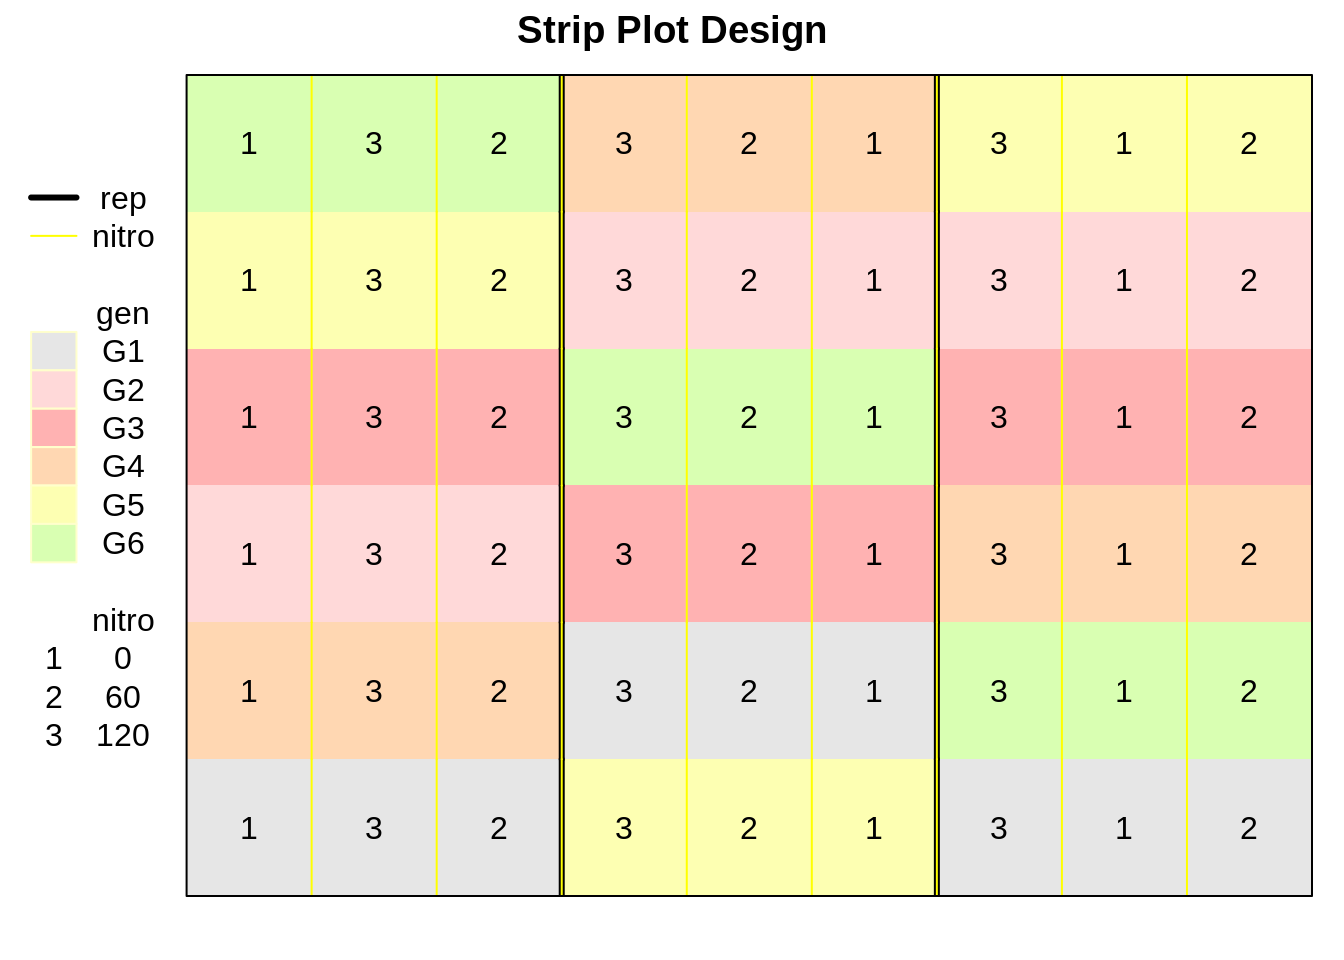
\includegraphics{./glmm_files/figure-pdf/unnamed-chunk-5-1.pdf}

}

\end{figure}

\begin{Shaded}
\begin{Highlighting}[]
\FunctionTok{ggplot}\NormalTok{(insect\_exp, }\FunctionTok{aes}\NormalTok{(}\AttributeTok{x =}\NormalTok{ sampling\_date, }\AttributeTok{y =}\NormalTok{ insect\_counts, }\AttributeTok{color =}\NormalTok{ treatment, }\AttributeTok{group =}\NormalTok{ plot)) }\SpecialCharTok{+}
  \FunctionTok{geom\_point}\NormalTok{(}\AttributeTok{size =} \DecValTok{2}\NormalTok{) }\SpecialCharTok{+}
  \FunctionTok{geom\_line}\NormalTok{() }\SpecialCharTok{+}
  \FunctionTok{theme\_classic}\NormalTok{()}
\end{Highlighting}
\end{Shaded}

\begin{figure}[H]

{\centering 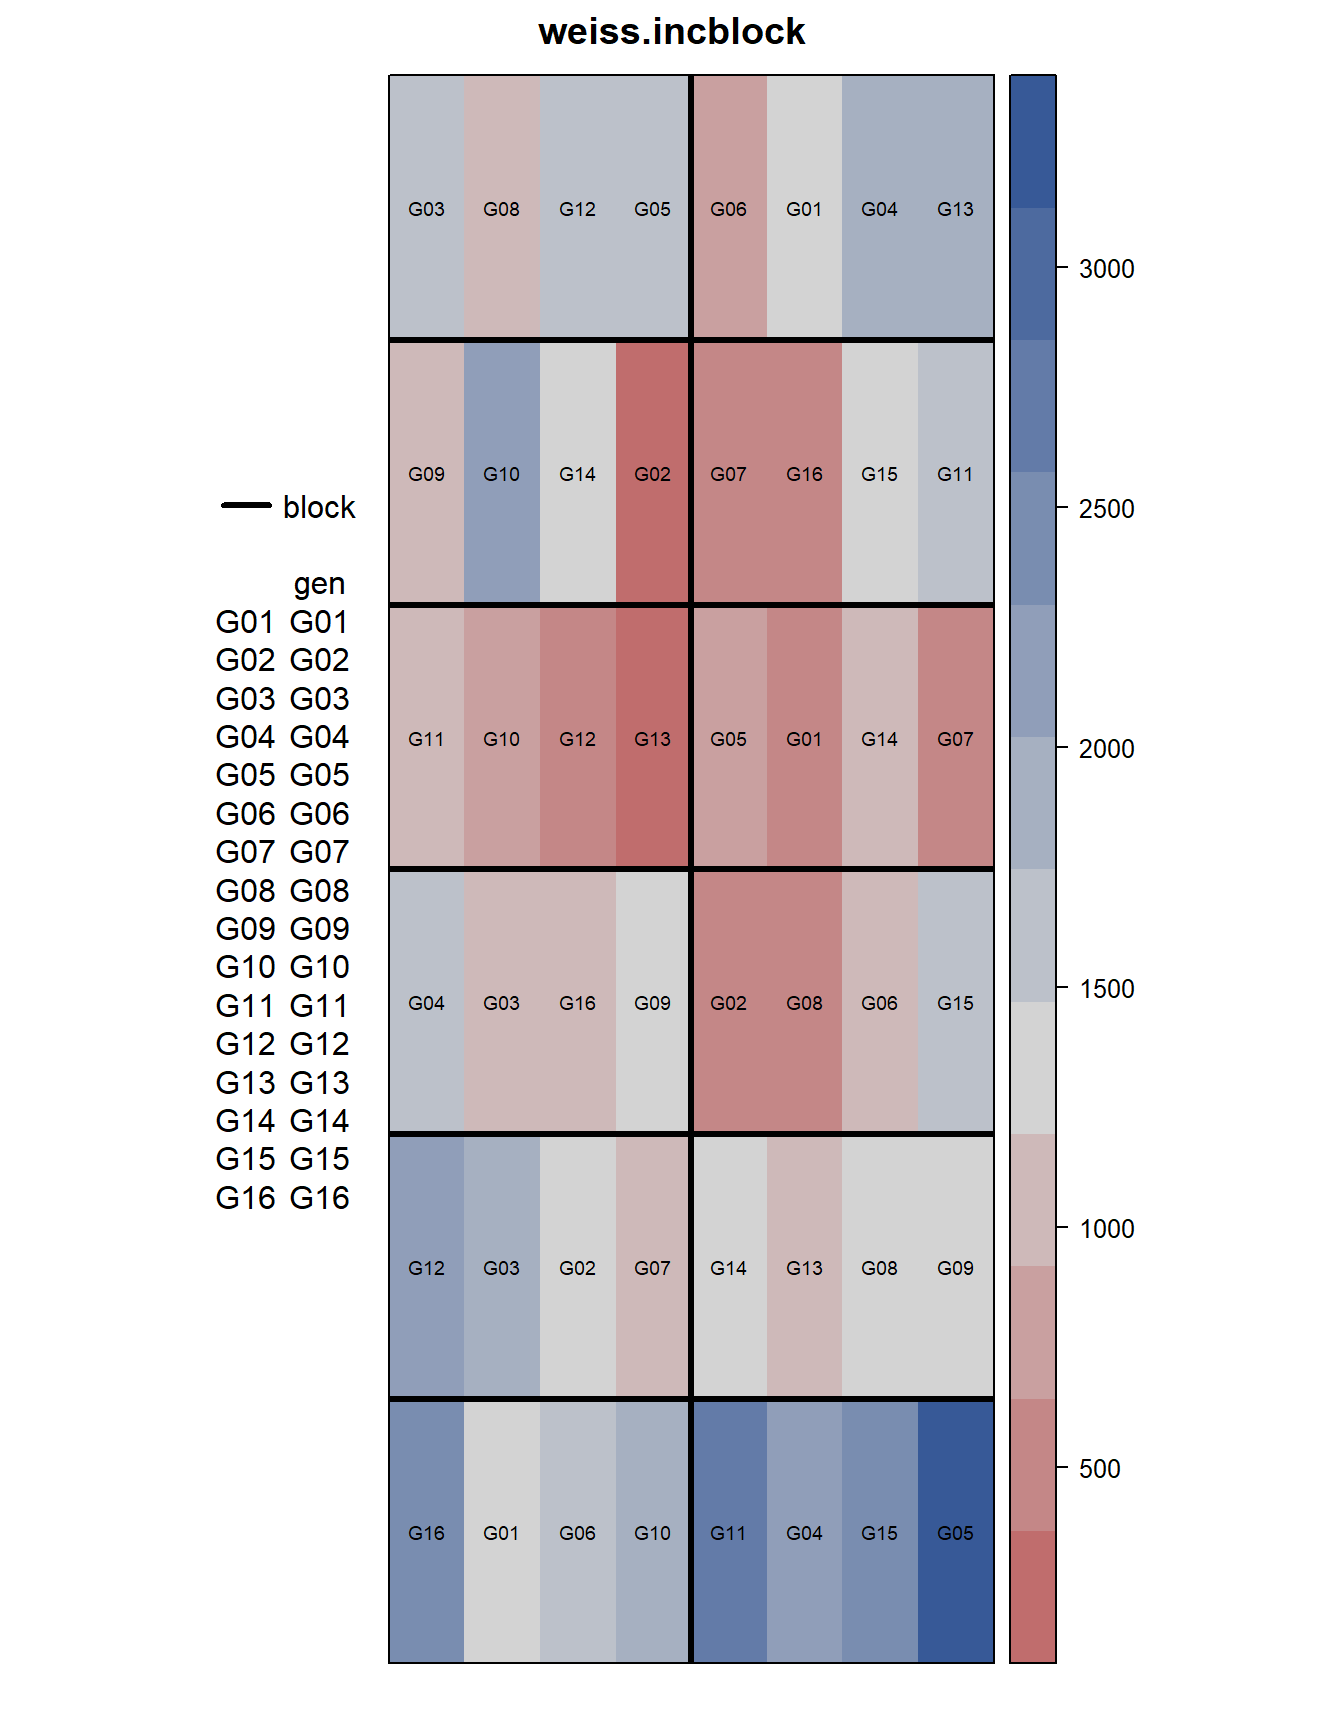
\includegraphics{./glmm_files/figure-pdf/unnamed-chunk-5-2.pdf}

}

\end{figure}

Model statement \{{[}{[}{[}{[} FIX THIS - it's still written for alfalfa
{]}{]}{]}{]}\}

\[y_{ijk} = \mu + \alpha_i+\beta_j + \gamma_k + a_l + b_m + c_n + \epsilon_{}\]
where

\(\mu\) = overall mean/intercept \(\alpha_i\) = effect of the \(i^{th}\)
pesticide treatment \(\beta_j\) = effect of the \(j^{th}\) block
\(\gamma_k\) = effect of the \(k^{th}\) sampling date

To make things easier, the interactions between the fixed effects are
not shown.

\begin{Shaded}
\begin{Highlighting}[]
\FunctionTok{library}\NormalTok{(glmmTMB)}

\NormalTok{m1 }\OtherTok{=} \FunctionTok{glmmTMB}\NormalTok{(}
\NormalTok{  insect\_counts }\SpecialCharTok{\textasciitilde{}}\NormalTok{ treatment }\SpecialCharTok{+}\NormalTok{ Date }\SpecialCharTok{+} \FunctionTok{ar1}\NormalTok{(Date }\SpecialCharTok{+} \DecValTok{0}\SpecialCharTok{|}\NormalTok{plot) }\SpecialCharTok{+}\NormalTok{ (}\DecValTok{1}\SpecialCharTok{|}\NormalTok{block),}
  \AttributeTok{ziformula =} \SpecialCharTok{\textasciitilde{}}\NormalTok{ treatment,}
  \AttributeTok{data =}\NormalTok{ insect\_exp, }\AttributeTok{na.action =}\NormalTok{ na.exclude, }
  \AttributeTok{family =}\NormalTok{ nbinom2)}
\end{Highlighting}
\end{Shaded}

special correlation structure for correlated error terms \texttt{ar1()}
(autoregressive 1).

There are several other specialized covariance structures implmented by
glmmTMB. In general, repeated measures syntax follow this convention:
\texttt{(time\ +\ 0\ \textbar{}\ grouping)}.

We can test other distributions

\begin{Shaded}
\begin{Highlighting}[]
\NormalTok{m2 }\OtherTok{\textless{}{-}} \FunctionTok{update}\NormalTok{(m1, }\AttributeTok{family =}\NormalTok{ poisson)}
\end{Highlighting}
\end{Shaded}

\begin{verbatim}
Warning in (function (start, objective, gradient = NULL, hessian = NULL, : NA/
NaN function evaluation

Warning in (function (start, objective, gradient = NULL, hessian = NULL, : NA/
NaN function evaluation

Warning in (function (start, objective, gradient = NULL, hessian = NULL, : NA/
NaN function evaluation

Warning in (function (start, objective, gradient = NULL, hessian = NULL, : NA/
NaN function evaluation
\end{verbatim}

\begin{verbatim}
Warning in fitTMB(TMBStruc): Model convergence problem; non-positive-definite
Hessian matrix. See vignette('troubleshooting')
\end{verbatim}

\begin{verbatim}
Warning in fitTMB(TMBStruc): Model convergence problem; false convergence (8).
See vignette('troubleshooting')
\end{verbatim}

\begin{Shaded}
\begin{Highlighting}[]
\NormalTok{m3 }\OtherTok{\textless{}{-}} \FunctionTok{update}\NormalTok{(m1, }\AttributeTok{family =}\NormalTok{ nbinom1)}
\end{Highlighting}
\end{Shaded}

\begin{verbatim}
Warning in (function (start, objective, gradient = NULL, hessian = NULL, : NA/
NaN function evaluation
\end{verbatim}

\begin{verbatim}
Warning in fitTMB(TMBStruc): Model convergence problem; non-positive-definite
Hessian matrix. See vignette('troubleshooting')
\end{verbatim}

\begin{verbatim}
Warning in fitTMB(TMBStruc): Model convergence problem; false convergence (8).
See vignette('troubleshooting')
\end{verbatim}

Fitting glmm is hard. Basic guidance on model fitting:
https://glmmtmb.github.io/glmmTMB/articles/troubleshooting.html

\begin{Shaded}
\begin{Highlighting}[]
\FunctionTok{diagnose}\NormalTok{(m2)}
\end{Highlighting}
\end{Shaded}

\begin{verbatim}
Unusually large Z-statistics (|x|>5):

    treatment3     treatment4     treatment5 Date1988-07-06 Date1988-07-13 
     -6.518478      -6.207956      -9.081474       9.422780       7.451213 
zi~(Intercept)  zi~treatment2 
     -5.166401     -10.640229 

Large Z-statistics (estimate/std err) suggest a *possible* failure of
the Wald approximation - often also associated with parameters that are
at or near the edge of their range (e.g. random-effects standard
deviations approaching 0).  (Alternately, they may simply represent
very well-estimated parameters; intercepts of non-centered models may
fall in this category.) While the Wald p-values and standard errors
listed in summary() may be unreliable, profile confidence intervals
(see ?confint.glmmTMB) and likelihood ratio test p-values derived by
comparing models (e.g. ?drop1) are probably still OK.  (Note that the
LRT is conservative when the null value is on the boundary, e.g. a
variance or zero-inflation value of 0 (Self and Liang 1987; Stram and
Lee 1994; Goldman and Whelan 2000); in simple cases these p-values are
approximately twice as large as they should be.)


Non-positive definite (NPD) Hessian

The Hessian matrix represents the curvature of the log-likelihood
surface at the maximum likelihood estimate (MLE) of the parameters (its
inverse is the estimate of the parameter covariance matrix).  A
non-positive-definite Hessian means that the likelihood surface is
approximately flat (or upward-curving) at the MLE, which means the
model is overfitted or poorly posed in some way. NPD Hessians are often
associated with extreme parameter estimates.


parameters with non-finite standard deviations:
(Intercept), zi~treatment5, theta_Date+0|plot.2, theta_1|block.1



recomputing Hessian via Richardson extrapolation. If this is too slow, consider setting check_hessian = FALSE 

Hessian has complex eigenvalues

We would have used the smallest eigenvalues of the Hessian to determine
which components were bad but instead we got complex eigenvalues. (Not
really sure what to do with this ...)
\end{verbatim}

\begin{Shaded}
\begin{Highlighting}[]
\FunctionTok{diagnose}\NormalTok{(m3)}
\end{Highlighting}
\end{Shaded}

\begin{verbatim}
Unusually large coefficients (|x|>10):

d~(Intercept) 
     -28.2372 

Large negative coefficients in zi (log-odds of zero-inflation),
dispersion, or random effects (log-standard deviations) suggest
unnecessary components (converging to zero on the constrained scale);
large negative and/or positive components in binomial or Poisson
conditional parameters suggest (quasi-)complete separation. Large
values of nbinom2 dispersion suggest that you should use a Poisson
model instead.


Unusually large Z-statistics (|x|>5):

    treatment5 Date1988-07-13  d~(Intercept) 
      -5.01654        9.85076    -2744.38790 

Large Z-statistics (estimate/std err) suggest a *possible* failure of
the Wald approximation - often also associated with parameters that are
at or near the edge of their range (e.g. random-effects standard
deviations approaching 0).  (Alternately, they may simply represent
very well-estimated parameters; intercepts of non-centered models may
fall in this category.) While the Wald p-values and standard errors
listed in summary() may be unreliable, profile confidence intervals
(see ?confint.glmmTMB) and likelihood ratio test p-values derived by
comparing models (e.g. ?drop1) are probably still OK.  (Note that the
LRT is conservative when the null value is on the boundary, e.g. a
variance or zero-inflation value of 0 (Self and Liang 1987; Stram and
Lee 1994; Goldman and Whelan 2000); in simple cases these p-values are
approximately twice as large as they should be.)


Non-positive definite (NPD) Hessian

The Hessian matrix represents the curvature of the log-likelihood
surface at the maximum likelihood estimate (MLE) of the parameters (its
inverse is the estimate of the parameter covariance matrix).  A
non-positive-definite Hessian means that the likelihood surface is
approximately flat (or upward-curving) at the MLE, which means the
model is overfitted or poorly posed in some way. NPD Hessians are often
associated with extreme parameter estimates.


parameters with non-finite standard deviations:
(Intercept), treatment3



recomputing Hessian via Richardson extrapolation. If this is too slow, consider setting check_hessian = FALSE 

Hessian has complex eigenvalues

We would have used the smallest eigenvalues of the Hessian to determine
which components were bad but instead we got complex eigenvalues. (Not
really sure what to do with this ...)
\end{verbatim}

Summary info

\begin{Shaded}
\begin{Highlighting}[]
\NormalTok{m1}
\end{Highlighting}
\end{Shaded}

\begin{verbatim}
Formula:          
insect_counts ~ treatment + Date + ar1(Date + 0 | plot) + (1 |      block)
Zero inflation:                 ~treatment
Data: insect_exp
      AIC       BIC    logLik  df.resid 
1298.7328 1385.0949 -625.3664       246 
Random-effects (co)variances:

Conditional model:
 Groups Name           Std.Dev. Corr      
 plot   Date1988-06-17 0.7748   0.49 (ar1)
 block  (Intercept)    0.3333             

Number of obs: 270 / Conditional model: plot, 30; block, 5

Dispersion parameter for nbinom2 family (): 1.76 

Fixed Effects:

Conditional model:
   (Intercept)      treatment2      treatment3      treatment4      treatment5  
       2.39231        -0.04978        -1.53159        -2.75395        -2.50652  
    treatment6  Date1988-06-22  Date1988-06-27  Date1988-06-29  Date1988-07-06  
      -1.48975         0.24054         0.26618         0.62692         1.17067  
Date1988-07-13  Date1988-07-21  Date1988-07-27  Date1988-08-03  
       0.83442         0.19962        -0.96749        -1.11938  

Zero-inflation model:
(Intercept)   treatment2   treatment3   treatment4   treatment5   treatment6  
     -2.608       -1.200        1.568        2.607        1.542        2.134  
\end{verbatim}

Diagnostics

Look at residuals over space

\begin{Shaded}
\begin{Highlighting}[]
\NormalTok{insect\_exp}\SpecialCharTok{$}\NormalTok{model\_resids }\OtherTok{\textless{}{-}} \FunctionTok{residuals}\NormalTok{(m1)}

\FunctionTok{ggplot}\NormalTok{(insect\_exp, }\FunctionTok{aes}\NormalTok{(}\AttributeTok{x =}\NormalTok{ row, }\AttributeTok{y =}\NormalTok{ column, }\AttributeTok{fill =}\NormalTok{ model\_resids)) }\SpecialCharTok{+}
  \FunctionTok{geom\_tile}\NormalTok{() }\SpecialCharTok{+} 
  \FunctionTok{facet\_wrap}\NormalTok{(}\AttributeTok{facets =} \FunctionTok{vars}\NormalTok{(Date), }\AttributeTok{nrow =} \DecValTok{3}\NormalTok{, }\AttributeTok{ncol =} \DecValTok{3}\NormalTok{) }\SpecialCharTok{+} 
  \FunctionTok{scale\_fill\_viridis\_c}\NormalTok{(}\AttributeTok{direction =} \SpecialCharTok{{-}}\DecValTok{1}\NormalTok{) }\SpecialCharTok{+} 
  \FunctionTok{theme\_minimal}\NormalTok{()}
\end{Highlighting}
\end{Shaded}

\begin{figure}[H]

{\centering 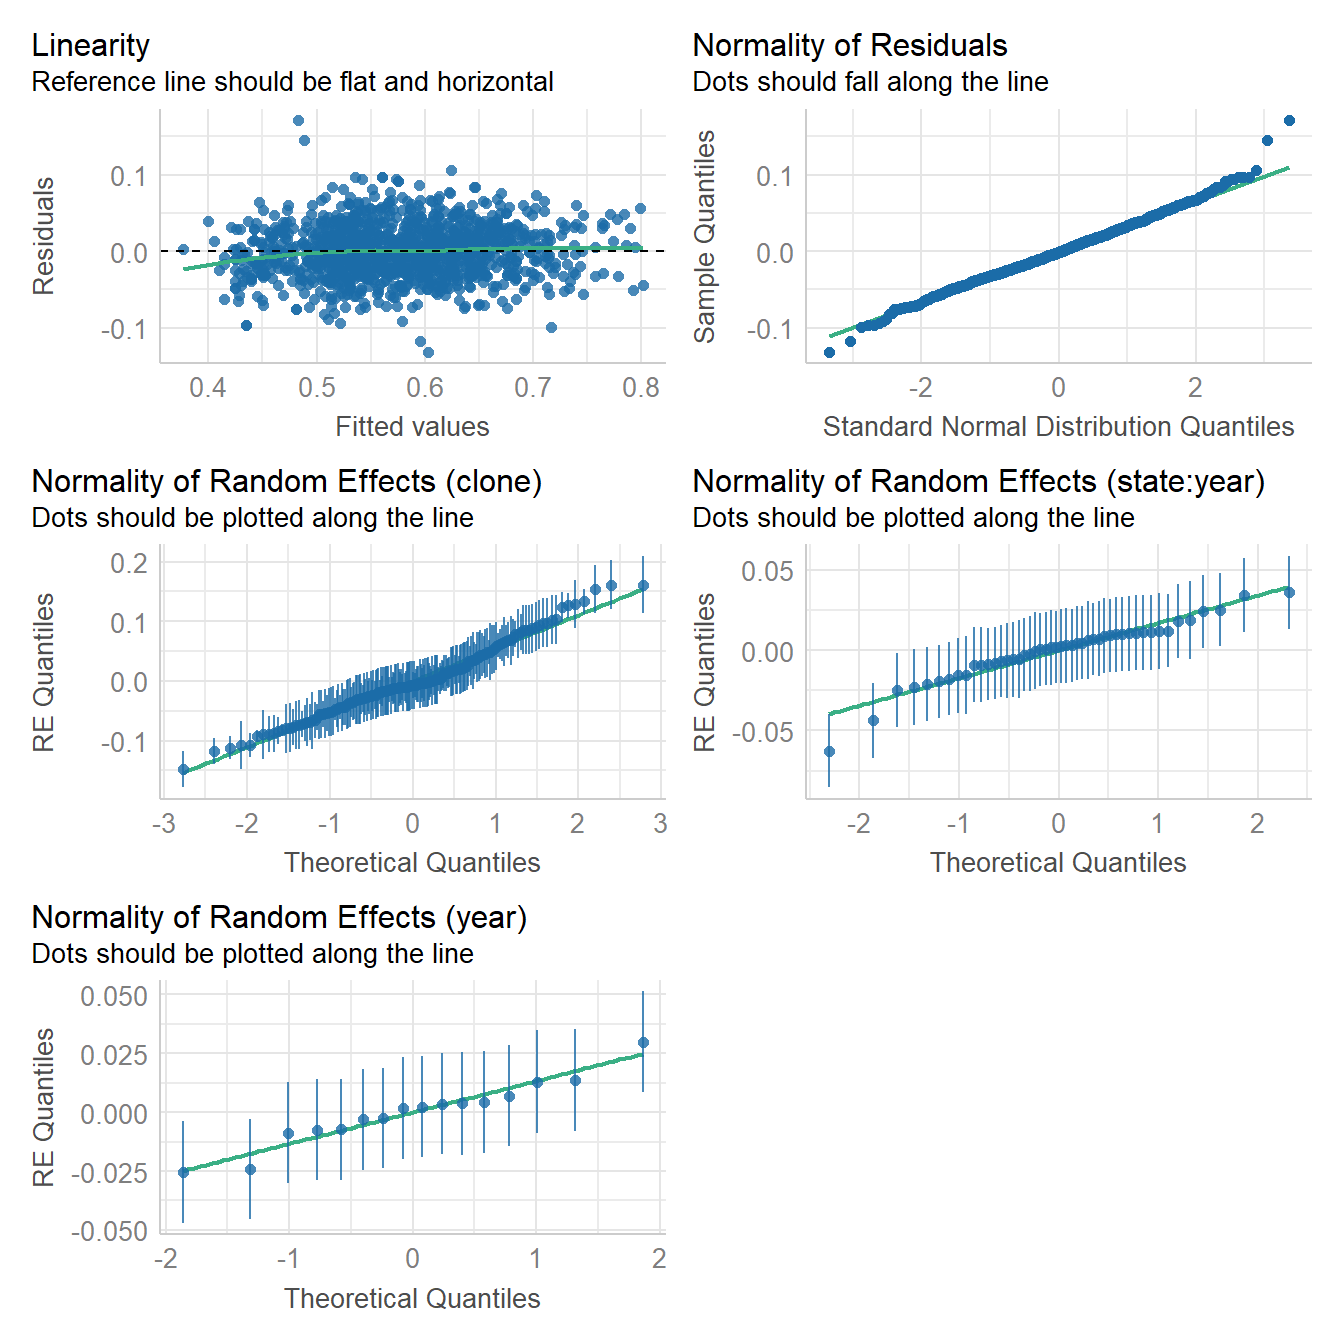
\includegraphics{./glmm_files/figure-pdf/unnamed-chunk-10-1.pdf}

}

\end{figure}

use \textbf{DHARMa} to conduct residual tests

\begin{Shaded}
\begin{Highlighting}[]
\NormalTok{simulated\_resids }\OtherTok{\textless{}{-}} \FunctionTok{simulateResiduals}\NormalTok{(m1)}
\FunctionTok{testDispersion}\NormalTok{(simulated\_resids)}
\end{Highlighting}
\end{Shaded}

\begin{figure}[H]

{\centering 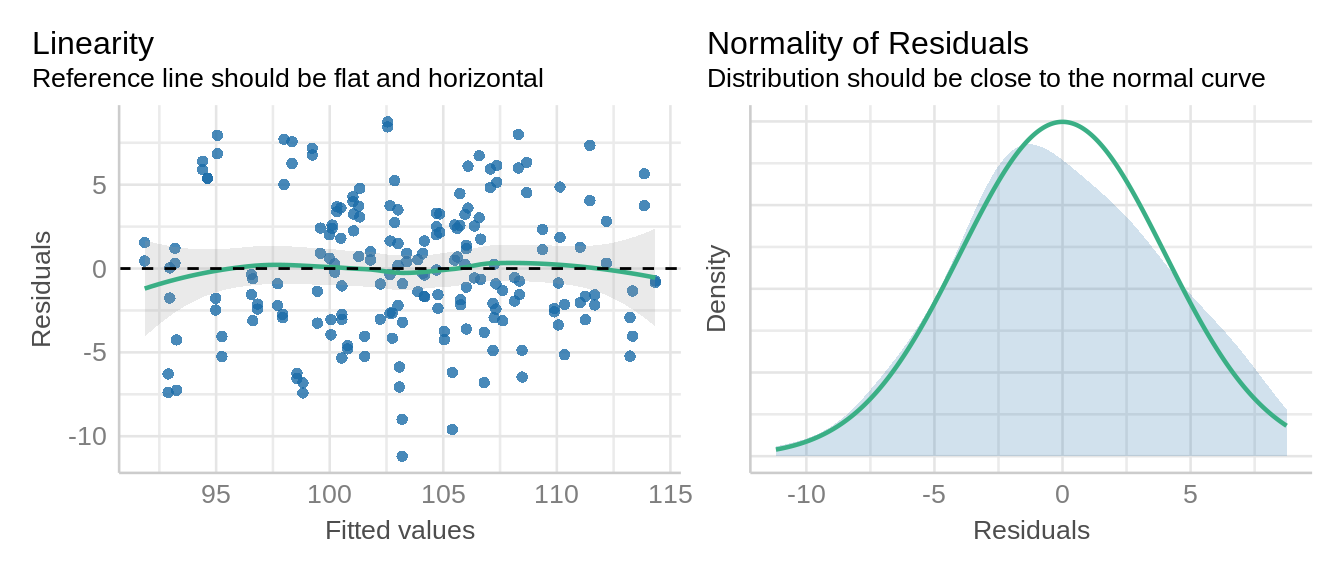
\includegraphics{./glmm_files/figure-pdf/unnamed-chunk-11-1.pdf}

}

\end{figure}

\begin{verbatim}

    DHARMa nonparametric dispersion test via sd of residuals fitted vs.
    simulated

data:  simulationOutput
dispersion = 0.23324, p-value = 0.336
alternative hypothesis: two.sided
\end{verbatim}

\begin{Shaded}
\begin{Highlighting}[]
\FunctionTok{plot}\NormalTok{(simulated\_resids)}
\end{Highlighting}
\end{Shaded}

\begin{figure}[H]

{\centering 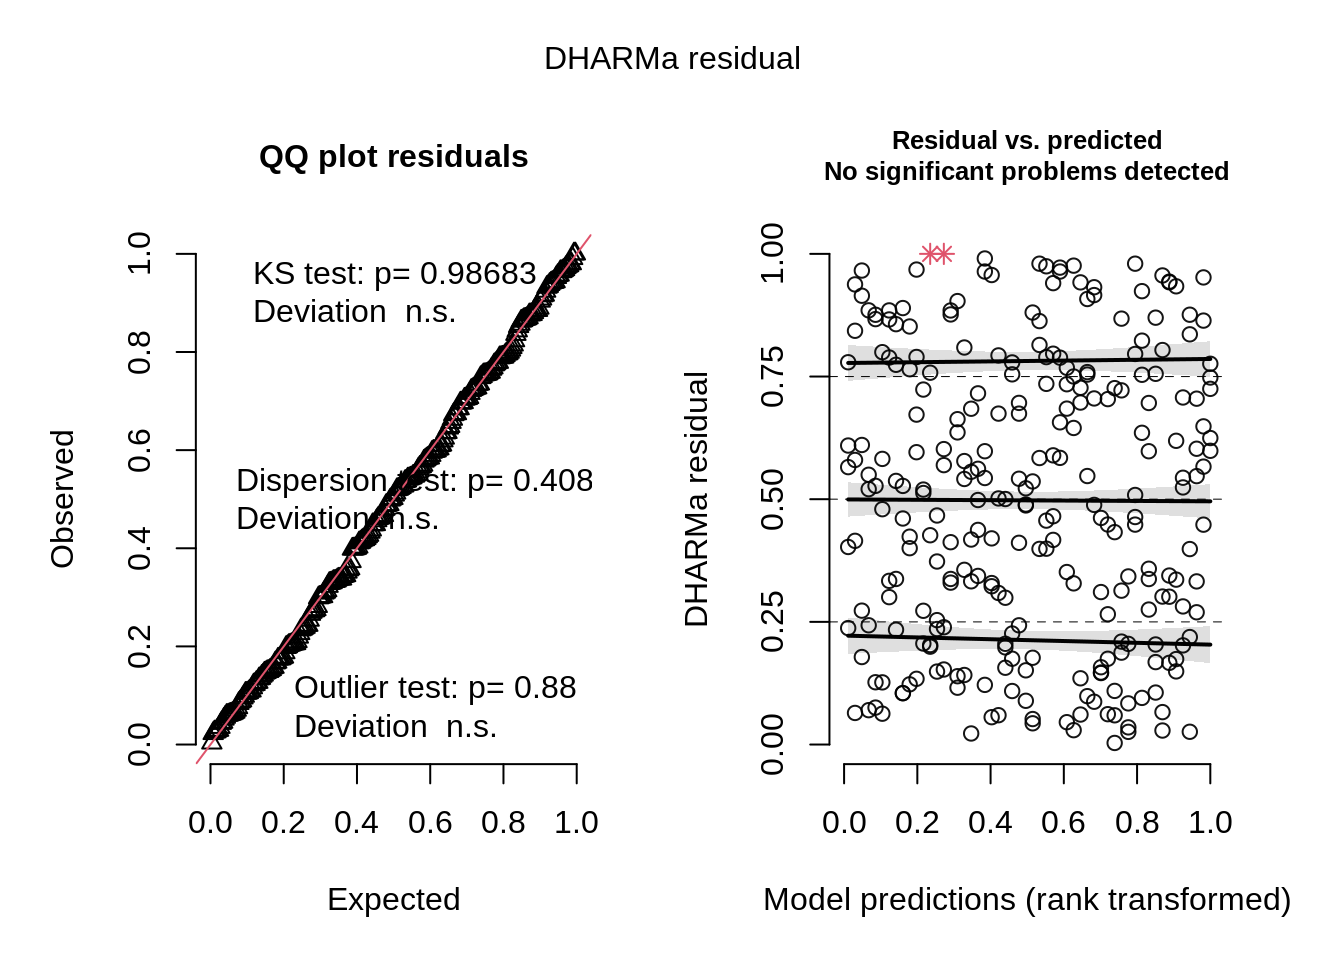
\includegraphics{./glmm_files/figure-pdf/unnamed-chunk-11-2.pdf}

}

\end{figure}

ANOVA

\begin{Shaded}
\begin{Highlighting}[]
\NormalTok{car}\SpecialCharTok{::}\FunctionTok{Anova}\NormalTok{(m1)}
\end{Highlighting}
\end{Shaded}

\begin{verbatim}
Analysis of Deviance Table (Type II Wald chisquare tests)

Response: insect_counts
           Chisq Df Pr(>Chisq)    
treatment 54.358  5  1.769e-10 ***
Date      41.652  8  1.574e-06 ***
---
Signif. codes:  0 '***' 0.001 '**' 0.01 '*' 0.05 '.' 0.1 ' ' 1
\end{verbatim}

\textbf{glmmTMB} is compatible with \textbf{emmeans} and
\textbf{effects}.

\bookmarksetup{startatroot}

\hypertarget{special-conditions}{%
\chapter{Special Conditions}\label{special-conditions}}

\hypertarget{split-plot-with-repeated-measures}{%
\section{Split plot with repeated
measures}\label{split-plot-with-repeated-measures}}

Main plot is ``irrigation'' and split plot is ``mix''.

\begin{Shaded}
\begin{Highlighting}[]
\NormalTok{alfalfa\_sp }\OtherTok{\textless{}{-}} \FunctionTok{read.csv}\NormalTok{(}\StringTok{"data/alfalfa2021\_data.csv"}\NormalTok{)}
\FunctionTok{library}\NormalTok{(dplyr)}
\end{Highlighting}
\end{Shaded}

\begin{verbatim}

Attaching package: 'dplyr'
\end{verbatim}

\begin{verbatim}
The following objects are masked from 'package:stats':

    filter, lag
\end{verbatim}

\begin{verbatim}
The following objects are masked from 'package:base':

    intersect, setdiff, setequal, union
\end{verbatim}

\textbf{cut}: a cutting (harvest) of alfalfa within a single growing
season. This is a temporal unit for repeated measures analysis. There
were three cuttings in total for that year and field. The dates are not
known, but we cannot assume they are evenly spaced apart.

\textbf{irrigation}: irrigation treatment (``Full'' or ``Deficit'')

\textbf{plot}: a unique number referring to each experimental unit

\textbf{block}: the blocking unit

\textbf{yield}: response variable

\textbf{row}: plot position for row

\textbf{col}: plot positions for column or range

\begin{Shaded}
\begin{Highlighting}[]
\FunctionTok{head}\NormalTok{(alfalfa\_sp)}
\end{Highlighting}
\end{Shaded}

\begin{verbatim}
    cut irrigation plot block     mix    yield row col
1 First       Full 1101     1 50A+50O 221.0418   1   1
2 First       Full 1102     1 75A+25O 288.7987   1   2
3 First       Full 1103     1 50A+50F 466.7924   1   3
4 First       Full 1104     1 75A+25M 556.9506   1   4
5 First       Full 1105     1 50A+50M 422.9160   1   5
6 First       Full 1106     1 75A+25F 289.8350   2   1
\end{verbatim}

Two new variables created:

\textbf{rep}: factor version of block (We should treat rep/block as a
factor rather than an integer in modelling)

\textbf{Cut}: number version of cut where 1 is the first cutting. This
is required by \texttt{nlme::lme} for specialized correlation
structures.

\begin{Shaded}
\begin{Highlighting}[]
\NormalTok{alfalfa\_sp }\OtherTok{\textless{}{-}}\NormalTok{ alfalfa\_sp }\SpecialCharTok{\%\textgreater{}\%} 
  \FunctionTok{mutate}\NormalTok{(}\AttributeTok{rep =} \FunctionTok{as.factor}\NormalTok{(block)) }\SpecialCharTok{\%\textgreater{}\%} 
  \FunctionTok{mutate}\NormalTok{(}\AttributeTok{Cut =} \FunctionTok{case\_when}\NormalTok{(}
\NormalTok{    cut }\SpecialCharTok{==} \StringTok{"First"} \SpecialCharTok{\textasciitilde{}}\NormalTok{ 1L,}
\NormalTok{    cut }\SpecialCharTok{==} \StringTok{"Second"} \SpecialCharTok{\textasciitilde{}}\NormalTok{ 2L,}
\NormalTok{    cut }\SpecialCharTok{==} \StringTok{"Third"} \SpecialCharTok{\textasciitilde{}}\NormalTok{ 3L,}
    \FunctionTok{is.na}\NormalTok{(cut) }\SpecialCharTok{\textasciitilde{}} \ConstantTok{NA\_integer\_}\NormalTok{)) }
\end{Highlighting}
\end{Shaded}

Visualise data

\begin{Shaded}
\begin{Highlighting}[]
\FunctionTok{library}\NormalTok{(ggplot2); }\FunctionTok{library}\NormalTok{(desplot)}

\NormalTok{alfalfa\_sp }\SpecialCharTok{\%\textgreater{}\%} \FunctionTok{filter}\NormalTok{(cut }\SpecialCharTok{==} \StringTok{"First"}\NormalTok{) }\SpecialCharTok{\%\textgreater{}\%} 
  
\FunctionTok{ggplot}\NormalTok{(}\FunctionTok{aes}\NormalTok{(}\AttributeTok{x =}\NormalTok{ col, }\AttributeTok{y =}\NormalTok{ row)) }\SpecialCharTok{+}
  \FunctionTok{geom\_raster}\NormalTok{(}\FunctionTok{aes}\NormalTok{(}\AttributeTok{fill =}\NormalTok{ irrigation)) }\SpecialCharTok{+}
  \FunctionTok{geom\_tileborder}\NormalTok{(}\FunctionTok{aes}\NormalTok{(}\AttributeTok{group =} \DecValTok{1}\NormalTok{, }\AttributeTok{grp =}\NormalTok{ rep), }\AttributeTok{lwd =} \FloatTok{1.5}\NormalTok{) }\SpecialCharTok{+} 
  \FunctionTok{theme\_classic}\NormalTok{()}
\end{Highlighting}
\end{Shaded}

\begin{figure}[H]

{\centering 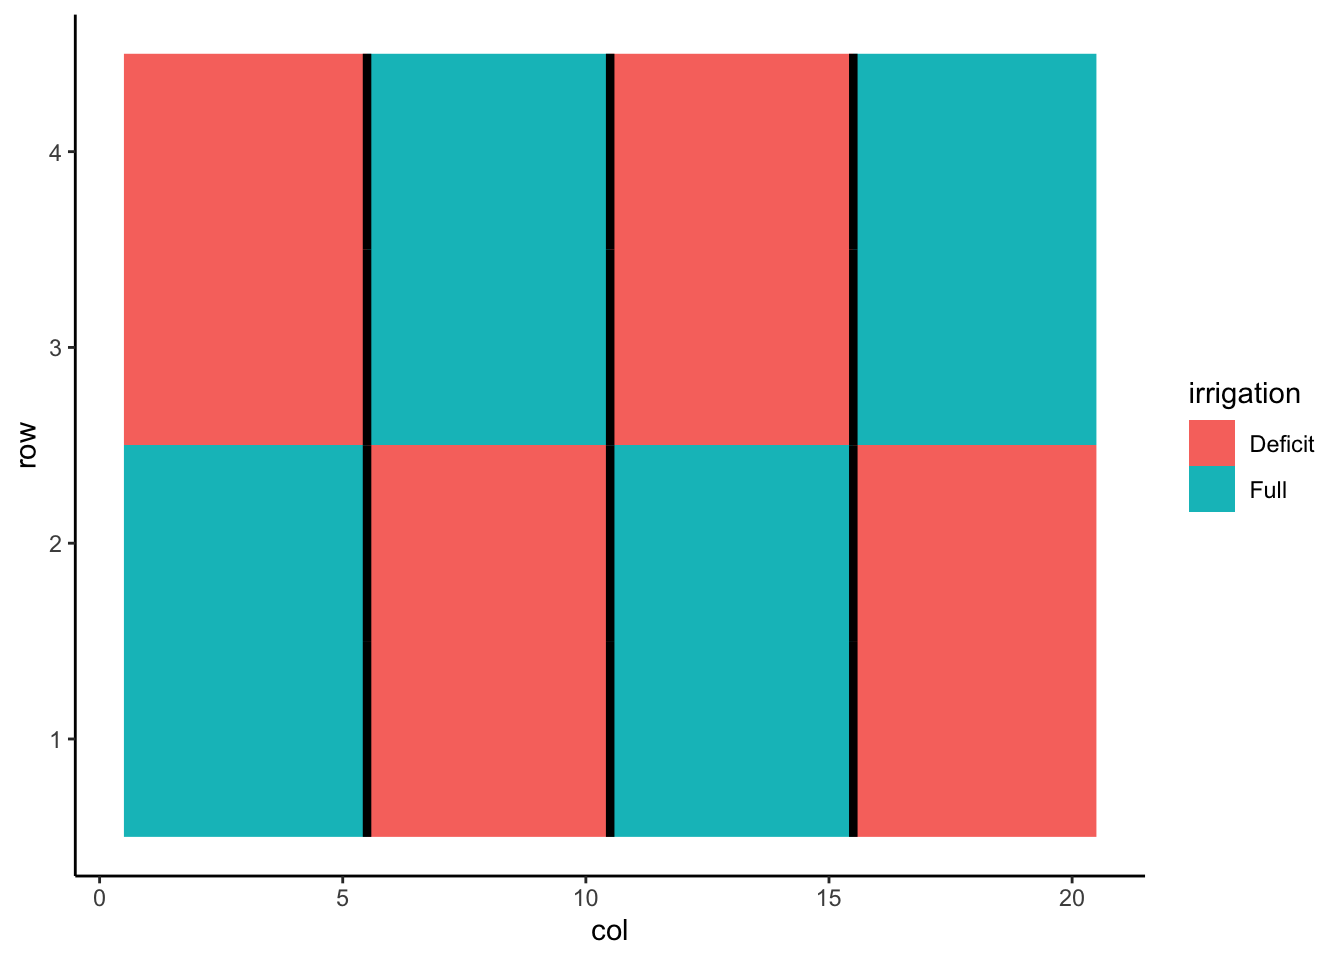
\includegraphics{./special_conditions_files/figure-pdf/unnamed-chunk-4-1.pdf}

}

\end{figure}

Model statement

\[y_{ijk} = \mu + \alpha_i+\beta_j + \gamma_k + a_l + b_m + c_n + \epsilon_{}\]
where

\(\mu\) = overall mean/intercept\\
\(\alpha_i\) = effect of the \(i^{th}\) irrigation treatment\\
\(\beta_j\) = effect of the \(j^{th}\) planting mix treatment
\(\gamma_k\) = effect of the \(k^{th}\) cutting {[}{[}need all those
interactions{]}{]}

\begin{Shaded}
\begin{Highlighting}[]
\FunctionTok{library}\NormalTok{(nlme)}
\end{Highlighting}
\end{Shaded}

\begin{verbatim}

Attaching package: 'nlme'
\end{verbatim}

\begin{verbatim}
The following object is masked from 'package:dplyr':

    collapse
\end{verbatim}

\begin{Shaded}
\begin{Highlighting}[]
\NormalTok{m1 }\OtherTok{\textless{}{-}} \FunctionTok{lme}\NormalTok{(yield }\SpecialCharTok{\textasciitilde{}}\NormalTok{ mix}\SpecialCharTok{*}\NormalTok{irrigation}\SpecialCharTok{*}\NormalTok{cut,}
          \AttributeTok{random =} \SpecialCharTok{\textasciitilde{}} \DecValTok{1}\SpecialCharTok{|}\NormalTok{plot}\SpecialCharTok{/}\NormalTok{rep}\SpecialCharTok{/}\NormalTok{irrigation,}
          \AttributeTok{data =}\NormalTok{ alfalfa\_sp)}
\end{Highlighting}
\end{Shaded}

use a special correlation structure for correlated error terms
\texttt{corCompSymm()} is for compound symmetry. There are several other
options in the \textbf{nlm} machinery (search ``cor'' for more options
and details on the syntax). In general, repeated measures syntax follow
this convention:
\texttt{form\ =\ \textasciitilde{}\ time\textbar{}grouping}. You can
also use \texttt{1\textbar{}group} and the observation order for each
group will be. The default starting value (\texttt{value}) is zero, and
if \texttt{fixed\ =\ FALSE} (the current nlme default), this value will
be allowed to change during the model fitting process.

\begin{Shaded}
\begin{Highlighting}[]
\NormalTok{corstr }\OtherTok{\textless{}{-}} \FunctionTok{corCompSymm}\NormalTok{(}\AttributeTok{value =} \FloatTok{0.3}\NormalTok{, }
                      \AttributeTok{form =} \SpecialCharTok{\textasciitilde{}}\NormalTok{ cut}\SpecialCharTok{|}\NormalTok{plot}\SpecialCharTok{/}\NormalTok{rep}\SpecialCharTok{/}\NormalTok{irrigation,}
                      \AttributeTok{fixed =} \ConstantTok{FALSE}\NormalTok{)}
\end{Highlighting}
\end{Shaded}

It's important that these two terms match after the ``\textbar{}'' in
the \texttt{random} and \texttt{form} arguments:

\begin{Shaded}
\begin{Highlighting}[numbers=left,,]
\NormalTok{m1 }\OtherTok{\textless{}{-}} \FunctionTok{lme}\NormalTok{(yield }\SpecialCharTok{\textasciitilde{}}\NormalTok{ mix}\SpecialCharTok{*}\NormalTok{irrigation}\SpecialCharTok{*}\NormalTok{cut,}
          \AttributeTok{random =} \SpecialCharTok{\textasciitilde{}} \DecValTok{1}\SpecialCharTok{|}\NormalTok{plot}\SpecialCharTok{/}\NormalTok{rep}\SpecialCharTok{/}\NormalTok{irrigation,}
          \AttributeTok{data =}\NormalTok{ alfalfa\_sp)}

\NormalTok{corstr }\OtherTok{\textless{}{-}} \FunctionTok{corCompSymm}\NormalTok{(}\AttributeTok{value =} \FloatTok{0.3}\NormalTok{, }
                      \AttributeTok{form =} \SpecialCharTok{\textasciitilde{}}\NormalTok{ cut}\SpecialCharTok{|}\NormalTok{plot}\SpecialCharTok{/}\NormalTok{rep}\SpecialCharTok{/}\NormalTok{irrigation,}
                      \AttributeTok{fixed =} \ConstantTok{FALSE}\NormalTok{)}
\end{Highlighting}
\end{Shaded}

Update the model:

\begin{Shaded}
\begin{Highlighting}[]
\NormalTok{m2 }\OtherTok{\textless{}{-}} \FunctionTok{update}\NormalTok{(m1, }\AttributeTok{cor =}\NormalTok{ corstr)}
\end{Highlighting}
\end{Shaded}

The usual next steps:

check diagnostics

\begin{Shaded}
\begin{Highlighting}[]
\FunctionTok{plot}\NormalTok{(m2)}
\end{Highlighting}
\end{Shaded}

\begin{figure}[H]

{\centering 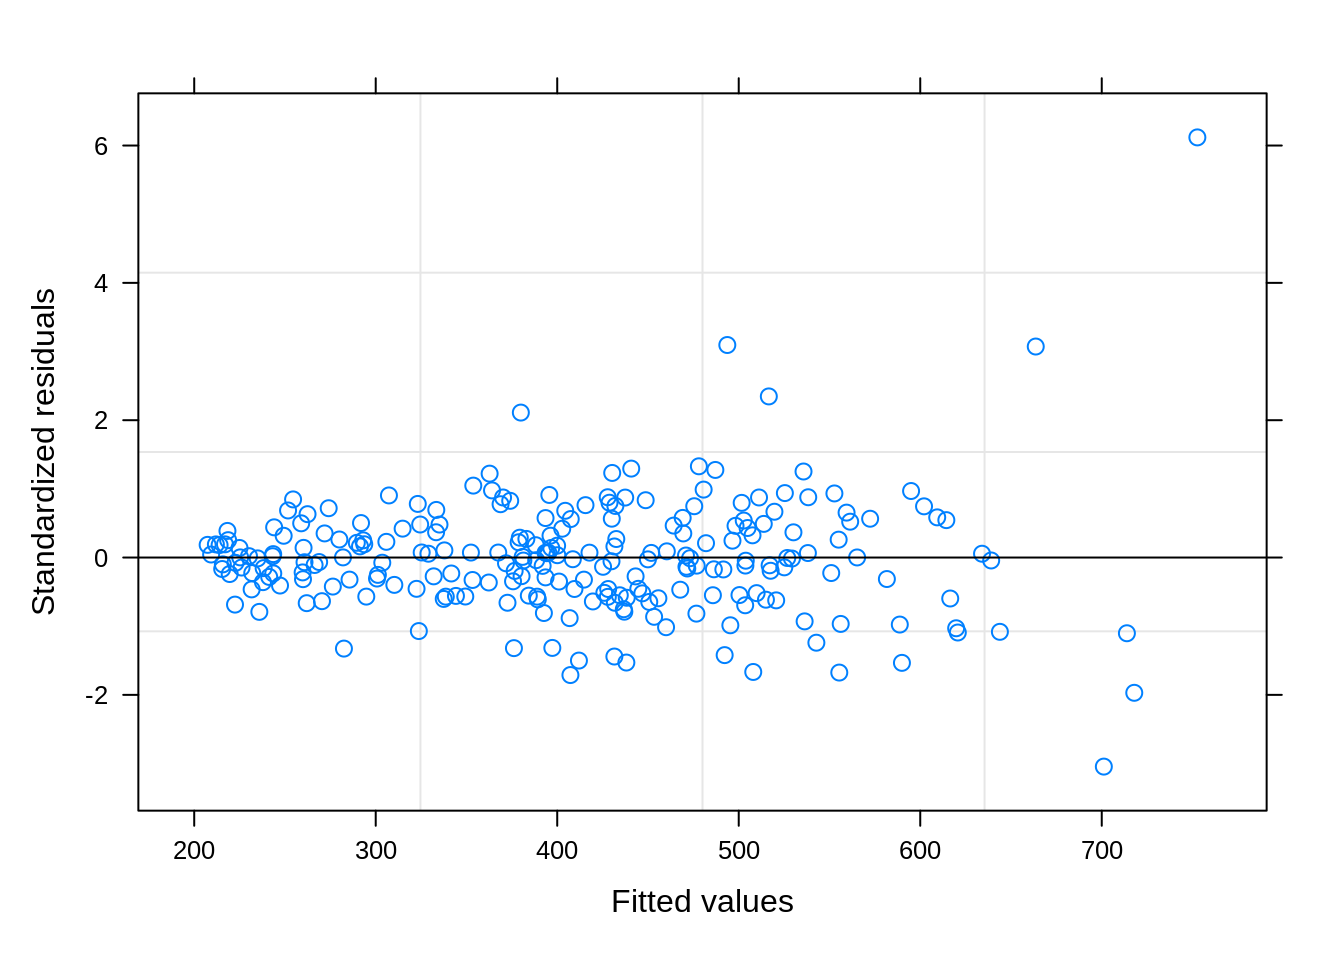
\includegraphics{./special_conditions_files/figure-pdf/unnamed-chunk-9-1.pdf}

}

\end{figure}

\begin{Shaded}
\begin{Highlighting}[]
\FunctionTok{qqnorm}\NormalTok{(m2, }\SpecialCharTok{\textasciitilde{}} \FunctionTok{resid}\NormalTok{(., }\AttributeTok{type =} \StringTok{"p"}\NormalTok{), }\AttributeTok{abline =} \FunctionTok{c}\NormalTok{(}\DecValTok{0}\NormalTok{, }\DecValTok{1}\NormalTok{))}
\end{Highlighting}
\end{Shaded}

\begin{figure}[H]

{\centering 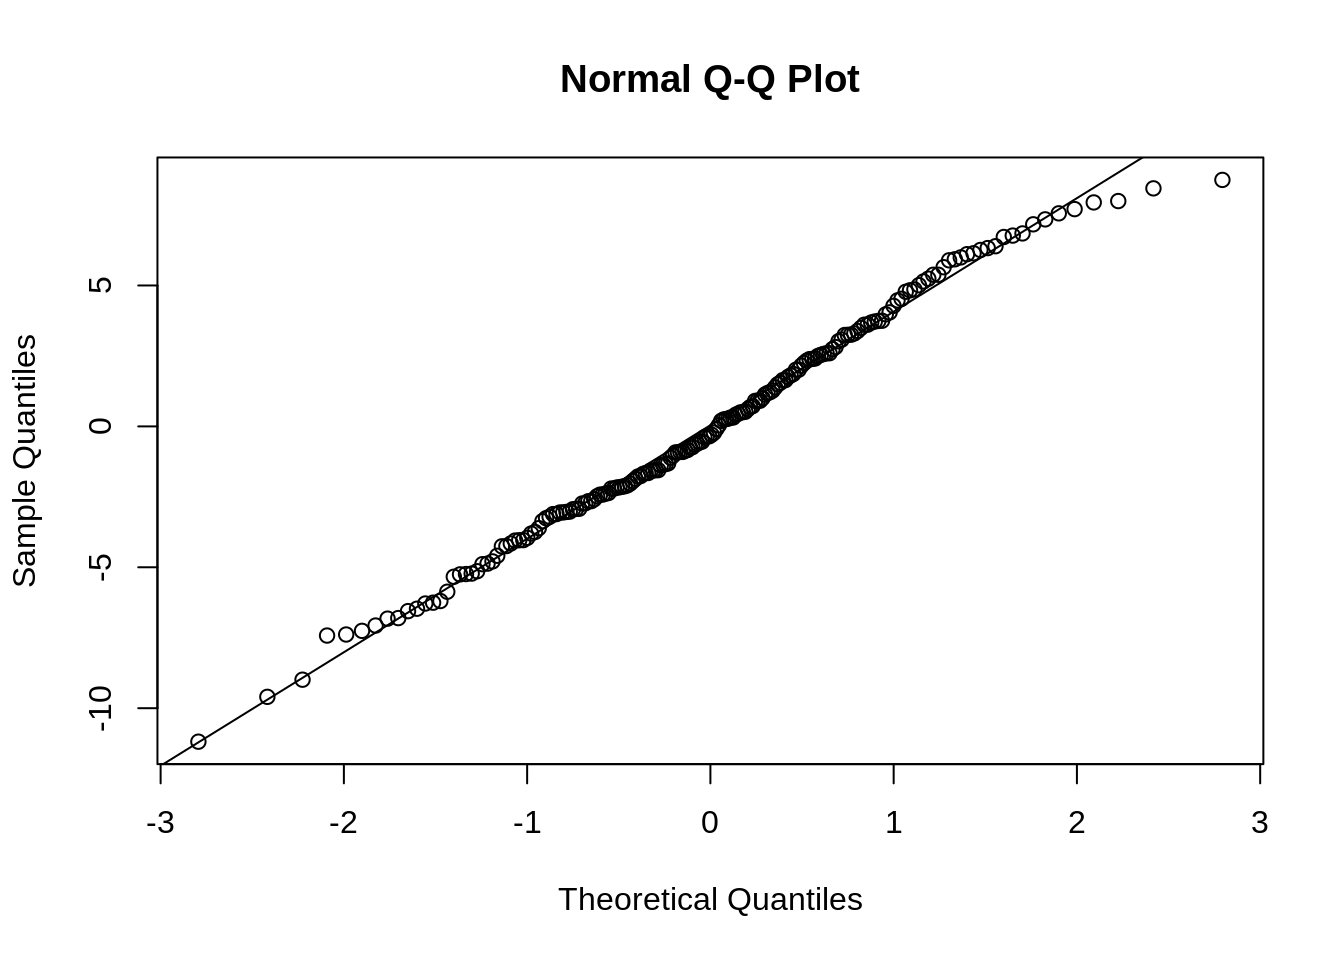
\includegraphics{./special_conditions_files/figure-pdf/unnamed-chunk-9-2.pdf}

}

\end{figure}

Look at the variance components.

\begin{Shaded}
\begin{Highlighting}[]
\FunctionTok{VarCorr}\NormalTok{(m2)}
\end{Highlighting}
\end{Shaded}

\begin{verbatim}
             Variance     StdDev   
plot =       pdLogChol(1)          
(Intercept)    287.6650    16.96069
rep =        pdLogChol(1)          
(Intercept)    287.6901    16.96143
irrigation = pdLogChol(1)          
(Intercept)    287.6733    16.96094
Residual     16164.7176   127.14054
\end{verbatim}

Run ANOVA

\begin{Shaded}
\begin{Highlighting}[]
\FunctionTok{anova}\NormalTok{(m2)}
\end{Highlighting}
\end{Shaded}

\begin{verbatim}
                   numDF denDF   F-value p-value
(Intercept)            1   102 2576.9579  <.0001
mix                    9   102   12.7163  <.0001
irrigation             1    78    7.1938  0.0089
cut                    2   102    6.0436  0.0033
mix:irrigation         9   102    0.4854  0.8814
mix:cut               18   102    0.8000  0.6960
irrigation:cut         2   102   14.2652  <.0001
mix:irrigation:cut    18   102    1.0220  0.4425
\end{verbatim}

always check the degrees of freedom (denominator and numerator)!

\bookmarksetup{startatroot}

\hypertarget{summary}{%
\chapter{Summary}\label{summary}}

In summary, mixed models are complicated.

\bookmarksetup{startatroot}

\hypertarget{references}{%
\chapter*{References}\label{references}}
\addcontentsline{toc}{chapter}{References}

\hypertarget{refs}{}
\begin{CSLReferences}{0}{0}
\end{CSLReferences}



\end{document}
